% This is "sig-alternate.tex" V2.1 April 2013
% This file should be compiled with V2.5 of "sig-alternate.cls" May 2012
%
% This example file demonstrates the use of the 'sig-alternate.cls'
% V2.5 LaTeX2e document class file. It is for those submitting
% articles to ACM Conference Proceedings WHO DO NOT WISH TO
% STRICTLY ADHERE TO THE SIGS (PUBS-BOARD-ENDORSED) STYLE.
% The 'sig-alternate.cls' file will produce a similar-looking,
% albeit, 'tighter' paper resulting in, invariably, fewer pages.
%
% ----------------------------------------------------------------------------------------------------------------
% This .tex file (and associated .cls V2.5) produces:
%       1) The Permission Statement
%       2) The Conference (location) Info information
%       3) The Copyright Line with ACM data
%       4) NO page numbers
%
% as against the acm_proc_article-sp.cls file which
% DOES NOT produce 1) thru' 3) above.
%
% Using 'sig-alternate.cls' you have control, however, from within
% the source .tex file, over both the CopyrightYear
% (defaulted to 200X) and the ACM Copyright Data
% (defaulted to X-XXXXX-XX-X/XX/XX).
% e.g.
% \CopyrightYear{2007} will cause 2007 to appear in the copyright line.
% \crdata{0-12345-67-8/90/12} will cause 0-12345-67-8/90/12 to appear in the copyright line.
%
% ---------------------------------------------------------------------------------------------------------------
% This .tex source is an example which *does* use
% the .bib file (from which the .bbl file % is produced).
% REMEMBER HOWEVER: After having produced the .bbl file,
% and prior to final submission, you *NEED* to 'insert'
% your .bbl file into your source .tex file so as to provide
% ONE 'self-contained' source file.
%
% ================= IF YOU HAVE QUESTIONS =======================
% Questions regarding the SIGS styles, SIGS policies and
% procedures, Conferences etc. should be sent to
% Adrienne Griscti (griscti@acm.org)
%
% Technical questions _only_ to
% Gerald Murray (murray@hq.acm.org)
% ===============================================================
%
% For tracking purposes - this is V2.0 - May 2012

\documentclass{sig-alternate-10pt}
%\documentclass{sig-alternate-05-2015}
\usepackage{url}
\usepackage{multirow}
% *** SUBFIGURE PACKAGES ***
%\ifCLASSOPTIONcompsoc
  \usepackage[caption=false,font=normalsize,labelfont=sf,textfont=sf]{subfig}
%\else
%  \usepackage[caption=false,font=footnotesize]{subfig}
%\fi

\begin{document}

% Copyright
%%%\setcopyright{acmcopyright}
%\setcopyright{acmlicensed}
%\setcopyright{rightsretained}
%\setcopyright{usgov}
%\setcopyright{usgovmixed}
%\setcopyright{cagov}
%\setcopyright{cagovmixed}


% DOI
%%%\doi{10.475/123_4}

% ISBN
%%%\isbn{123-4567-24-567/08/06}

%Conference
\conferenceinfo{PLDI '13}{June 16--19, 2013, Seattle, WA, USA}

%%%\acmPrice{\$15.00}

%
% --- Author Metadata here ---
\conferenceinfo{WOODSTOCK}{'97 El Paso, Texas USA}
%\CopyrightYear{2007} % Allows default copyright year (20XX) to be over-ridden - IF NEED BE.
%\crdata{0-12345-67-8/90/01}  % Allows default copyright data (0-89791-88-6/97/05) to be over-ridden - IF NEED BE.
% --- End of Author Metadata ---

%\title{Alternate {\ttlit ACM} SIG Proceedings Paper in LaTeX
%Format\titlenote{(Produces the permission block, and
%copyright information). For use with
%SIG-ALTERNATE.CLS. Supported by ACM.}}
%\subtitle{[Extended Abstract]
%\titlenote{A full version of this paper is available as
%\textit{Author's Guide to Preparing ACM SIG Proceedings Using
%\LaTeX$2_\epsilon$\ and BibTeX} at
%\texttt{www.acm.org/eaddress.htm}}}

\title{NI: A Benchmark Suite for NfvInsight}

%
% You need the command \numberofauthors to handle the 'placement
% and alignment' of the authors beneath the title.
%
% For aesthetic reasons, we recommend 'three authors at a time'
% i.e. three 'name/affiliation blocks' be placed beneath the title.
%
% NOTE: You are NOT restricted in how many 'rows' of
% "name/affiliations" may appear. We just ask that you restrict
% the number of 'columns' to three.
%
% Because of the available 'opening page real-estate'
% we ask you to refrain from putting more than six authors
% (two rows with three columns) beneath the article title.
% More than six makes the first-page appear very cluttered indeed.
%
% Use the \alignauthor commands to handle the names
% and affiliations for an 'aesthetic maximum' of six authors.
% Add names, affiliations, addresses for
% the seventh etc. author(s) as the argument for the
% \additionalauthors command.
% These 'additional authors' will be output/set for you
% without further effort on your part as the last section in
% the body of your article BEFORE References or any Appendices.

%\numberofauthors{5} %  in this sample file, there are a *total*
%% of EIGHT authors. SIX appear on the 'first-page' (for formatting
%% reasons) and the remaining two appear in the \additionalauthors section.
%%
%\author{
%% You can go ahead and credit any number of authors here,
%% e.g. one 'row of three' or two rows (consisting of one row of three
%% and a second row of one, two or three).
%%
%% The command \alignauthor (no curly braces needed) should
%% precede each author name, affiliation/snail-mail address and
%% e-mail address. Additionally, tag each line of
%% affiliation/address with \affaddr, and tag the
%% e-mail address with \email.
%%
%% 1st. author
%\alignauthor
%Ben Trovato\titlenote{Dr.~Trovato insisted his name be first.}\\
%       \affaddr{Institute for Clarity in Documentation}\\
%       \affaddr{1932 Wallamaloo Lane}\\
%       \affaddr{Wallamaloo, New Zealand}\\
%       \email{trovato@corporation.com}
%% 2nd. author
%\alignauthor
%G.K.M. Tobin\titlenote{The secretary disavows
%any knowledge of this author's actions.}\\
%       \affaddr{Institute for Clarity in Documentation}\\
%       \affaddr{P.O. Box 1212}\\
%       \affaddr{Dublin, Ohio 43017-6221}\\
%       \email{webmaster@marysville-ohio.com}
%% 3rd. author
%\alignauthor Lars Th{\o}rv{\"a}ld\titlenote{This author is the
%one who did all the really hard work.}\\
%       \affaddr{The Th{\o}rv{\"a}ld Group}\\
%       \affaddr{1 Th{\o}rv{\"a}ld Circle}\\
%       \affaddr{Hekla, Iceland}\\
%       \email{larst@affiliation.org}
%\and  % use '\and' if you need 'another row' of author names
%% 4th. author
%\alignauthor Lawrence P. Leipuner\\
%       \affaddr{Brookhaven Laboratories}\\
%       \affaddr{Brookhaven National Lab}\\
%       \affaddr{P.O. Box 5000}\\
%       \email{lleipuner@researchlabs.org}
%% 5th. author
%\alignauthor Sean Fogarty\\
%       \affaddr{NASA Ames Research Center}\\
%       \affaddr{Moffett Field}\\
%       \affaddr{California 94035}\\
%       \email{fogartys@amesres.org}
%}

% There's nothing stopping you putting the seventh, eighth, etc.
% author on the opening page (as the 'third row') but we ask,
% for aesthetic reasons that you place these 'additional authors'
% in the \additional authors block, viz.
%\additionalauthors{Additional authors: John Smith (The Th{\o}rv{\"a}ld Group,
%email: {\texttt{jsmith@affiliation.org}}) and Julius P.~Kumquat
%(The Kumquat Consortium, email: {\texttt{jpkumquat@consortium.net}}).}
%\date{30 July 1999}
% Just remember to make sure that the TOTAL number of authors
% is the number that will appear on the first page PLUS the
% number that will appear in the \additionalauthors section.

\maketitle
\begin{abstract}
NFV is attracting more and more interest in both industry and academia. 
It is promising to reduce cost for network operators and accelerate innovation 
by replacing traditional hardware-base appliance with virtualized functions 
deployed in cloud computing environment.
NFV testing environment deploying 
involves multiple layers in the software stack including 
VNF image packaging, virtualization management, 
network configuration, forwarding rule installation, 
and performance metric measurement. 
According to our survey, 
it takes averagely 1-2 human-month to set up a testing environment.
Motivated by the time taking process of deployment, 
we decided to develop an easy-to-use NFV benchmark named NI.
The benchmark has three key features: 
1) Representative NFs 
2) One-click running 
3) Plenty metrics for measurement. 
NI includes 5 VNF %covering half of the NFV use cases, 
and provides typical NF chaining policies. 
NI leverages Kubernetes and Docker to do infrastructure management, 
and OVS to control data flow. 
Our evaluation shows measurement results NI can provide.
\end{abstract}


%
% The code below should be generated by the tool at
% http://dl.acm.org/ccs.cfm
% Please copy and paste the code instead of the example below. 
%
%%%\begin{CCSXML}
%%%<ccs2012>
%%% <concept>
%%%  <concept_id>10010520.10010553.10010562</concept_id>
%%%  <concept_desc>Computer systems organization~Embedded systems</concept_desc>
%%%  <concept_significance>500</concept_significance>
%%% </concept>
%%% <concept>
%%%  <concept_id>10010520.10010575.10010755</concept_id>
%%%  <concept_desc>Computer systems organization~Redundancy</concept_desc>
%%%  <concept_significance>300</concept_significance>
%%% </concept>
%%% <concept>
%%%  <concept_id>10010520.10010553.10010554</concept_id>
%%%  <concept_desc>Computer systems organization~Robotics</concept_desc>
%%%  <concept_significance>100</concept_significance>
%%% </concept>
%%% <concept>
%%%  <concept_id>10003033.10003083.10003095</concept_id>
%%%  <concept_desc>Networks~Network reliability</concept_desc>
%%%  <concept_significance>100</concept_significance>
%%% </concept>
%%%</ccs2012>  
%%%\end{CCSXML}

%%%\ccsdesc[500]{Computer systems organization~Embedded systems}
%%%\ccsdesc[300]{Computer systems organization~Redundancy}
%%%\ccsdesc{Computer systems organization~Robotics}
%%%\ccsdesc[100]{Networks~Network reliability}


%
% End generated code
%

%
%  Use this command to print the description
%
%%%\printccsdesc

% We no longer use \terms command
%\terms{Theory}

\keywords{Network Function Virtualization; }

\section{Introduction}

Network function virtualization (NFV) has become a hot topic, both in industry and academia. Since the publication of NFV Introductory White Paper \cite{} of ETSI in 2012, a lot of works have been emerged in this field. Modification works of NFV were done on the whole software stack (or maybe both SW and HW stack?). There are de facto industrial NFV platform OPNFV \cite{noauthor_home_nodate} as well as advanced NF allocation frameworks like OpenNF \cite{gember-jacobson_opennf:_2014}, CoMb \cite{180672} and E2 \cite{palkar_e2:_2015}. Also, there are works like OpenBox \cite{bremler-barr_openbox:_2016} and Netbricks \cite{199352} to rewrite or modify the NFs.

%Embark\cite{194934}
%StateAlyzer\cite{194932}
%Split/Merge\cite{180307}
%ClickOS\cite{179771}
%APLOMB\cite{sherry_making_2012}
%FTMB\cite{sherry_rollback-recovery_2015}
%DFC\cite{194970}

However, a suite of easy-to-use NFV benchmark is not yet existed. It is unavoidable to experience a time consuming process finding both open source software and proper chaining policies. According to our observation, most NFs used in papers are different open source implementations linked in different kinds of NF chain policies. So that, there is not yet a general baseline for measurement and comparison. Furthermore, the workload generator and network traffic trace used are also different, traces need to be provided to test different NF chains.

We also did a survey among top conference researchers who have experiences setting up NFV environment. In our survey, we found that the deploying time varies much due to the scale. In average, it takes 1-2 months to build up a NF cluster having less than 10 VM instances. But when the scale of instances increase to over 50, the build up process can take 3-4 months or more. One of our respondent said that they were still keeping on iterating and improving their testbed constantly.



In this paper, we develop a suite of NF benchmarks, which is supposed to have the following characteristics: 1) Representing typical NFs 2) Easy to use 3) Plenty metrics for measurement.

According to our research and observation, 
the representative of an NFV benchmark 
should be satisfied in three aspects:
%\begin{itemize}
%\begin{enumerate}
%\item{\textbf{Representative NFs.}}
\textbf{1) Representative NFs.}
For the demand of representative NFs, 
we referred to the NFV Introductory White Paper \cite{}, 
which defined ten scenario of NFV use cases. 
In the first version of our benchmark, 
the open source implementation of NFs we collected 
covers half of the ten use cases. 
Table \ref{nfs} lists the basic information of NFs used in our benchmark. 
%\item{\textbf{Representative NF chains.}}
\textbf{2) Representative NF chains.}
However, not only single NFs should be typical, but also the NF chains. 
We referred to ETSI standard documents of SFC 
(Service Function Chaining) \cite{draft-ietf-sfc-dc-use-cases-06} 
for the typical use case of service chains 
in the scenarios of both enterprise user and datacenter.
We also consulted our industrial partners for real world chaining policies. 
The typical NF chains our benchmark provides are listed in Table \ref{chains}. 
%\item{\textbf{Proper workload generator.}} 
\textbf{3) Proper workload generator.}
Since each NF chain serves at different network level, 
only one workload generator is not enough to test all the scenarios. 
So we select different clients for each chain.
%and fixed the content of each chain.
%\end{itemize}
%\end{enumerate}


The goal of the `easy to use' design is to 
achieve one-week setting up as well as one-click test running, 
no matter the scale of the testing environment. 
To finish a test, users only need to touch one configuration file 
and execute one single command. 
In the end, the measurement report will be output to a file.
To implement our design, 
we leverage Docker and Kubernets to pack NFs in docker, 
manage the images, and do allocation automatically. 
We use OVS to do switching and packet force forwarding.
Pre-written scripts and Openflow rules are written 
to implement chaining and flow control. 
%There are more complains pointing out their pain points: 1) Automate the setting up and testing process. 2) Configure and stabilize NFs (?). 3) Write rules to set up topology and enforce flow control.
%%our design to solve the pain points????
%`easy to use' design should solve pain points

In our benchmark, we provide the most concerned metrics for measurement, 
that is latency and throughput. 
We measure latency in the granularity of per-packet and per-NF, 
and output cumulative distribution of latency in the measurement report. 

%The main contribution of our work is 

%\section{Background and Motivation}
%
%\subsection{Network Function Virtualization}
%NFV involves multi-layers in the whole software stack, 
%
%The concept of NFV chain

\section{A Survey of NFV Testing Environment Deploying}
%To further prove our observation, 
To get first-hand information about researchers' experience on 
NFV testing environment deploying, 
we did a survey among top conference authors 
dedicated in the field of NFV. 
We delivered the survey to sixteen people 
who are the first authors of their papers %published on top conferences 
and we finally collected eight responses. 

In the first place, we asked for the number of types of VNF they used, 
and the source of VNF, chaining policy and workload generator. 
Averagely, six types of VNF are used in one paper. 
Most of the VNF are open source implementations, 
though three of our respondents have written their own VNF. 
%a list of open source NFs found in papers??
The chaining policies are all find in papers or public policies. 
And for the workload generator, 
half of them directly used open source software, 
and half of them wrote by themselves.
%need some conclusion?

Another question we concerned most is 
the time they spent on deploying a NFV testing environment. 
To more precisely measure the labor time, 
we use the metric of man-month 
which indicates the number of months used 
if the work is done by one person. 
We also asked for the scale of physical servers and VM instances, 
as well as the virtualization technology they used. 
The result is shown in Table \ref{survey}.

\begin{table}[!t]
\newcommand{\tabincell}[2]{\begin{tabular}{@{}#1@{}}#2\end{tabular}}
\centering
\begin{tabular}{|c|c|c|c|c|}\hline
& \tabincell{c}{Man-Month\\Used} & \tabincell{c}{\# of\\Servers} & \tabincell{c}{\# of\\VMs} & \tabincell{c}{Virtualization\\Technology}\\\hline
1 & $<$0.5 & 4 & 11-20 & KVM\\\hline
2 & 0.5-1 & 2 & 1-5 & Hyper-V\\\hline
3 & 0.5-1 & 4 & 1-7 & Container\\\hline
4 & 0.5-1 & 4 & 6-10 & KVM\\\hline
5 & 1-2 & 4 & 6-10 & \tabincell{c}{Container,\\KVM and other}\\\hline
6 & 4 & 10 & 100 & KVM\\\hline
7 & 3 & 24 & 72 & KVM\\\hline
8 & \tabincell{c}{Constantly\\Iterating} & 4 & 1-5 & Xen\\\hline
\end{tabular}
\caption{The result of our survey reflects the relationship 
between labor consuming and the scale of the testing environment.}
\label{survey}
\end{table}

From the responses, we can see the average time 
to deploy a testing environment for NFV is around 1-2 months 
for a cluster not in very large scale.
It can be quite fast for a experienced person, 
as the responser No.1, who used less than half a month 
setting up a cluster including 4 physical servers and 11-20 VMs. 
However, for the others, the deploying process 
can be time taking and painful.
Take respondent No.6 and No.7 as examples, 
they built their test environment in quite large scale,
and it results in much longer setting up time. 

NFV setting up involves multi-layers in the whole software stack, 
which includes virtualization, cluster management, 
network virtualization, and NF configuration, 
so that any point can become a bottleneck, 
especially for a green hand. 
Take respondent No.8 as an example, 
Most problems they encountered are related to the hypervisor they used. 
And respondent No.7 said they changed from Xen 
to KVM with Openstack and things got much better.
We asked the authors for their most painful experiences, 
and we summarize the reasons making the setting up time so long 
as the following: 

\begin{itemize}
\item[-]{}
Automating the process of setting up the testbed. 
\item[-]{}
Setting up the datapath (interfaces, DPDK, routing tables, etc).
\item[-]{}
Installing proper rules in OpenFlow-enabled switches to enforce chaining.
\item[-]{}
Figure out appropriate workload to test different types of VNFs.
\item[-]{}
Figuring out how to determine that NFs were done starting up and ready to forward packets. 
\end{itemize}

%Automating the process of setting up the testbed end to end took us a lot of time and many iterations.
%%No.4
%
%We wrote a bunch of scripts that simplified most of the process. The primary trouble was in figuring out how to determine that NFs were done starting up and ready to forward packets.
%
%Two parts for me:
%1. Install, configure and stabilize the open-source software, especially under heavy workload.
%2. Figure out appropriate workload to test different types of VNFs. It would be great if there is some real-world traffic/workload traces.
%
%Traffic generation and topology configuration
%
%Setting up the datapath (interfaces, DPDK, routing tables, etc)
%Installing proper rules in OpenFlow-enabled switches to enforce chaining

One of our responser pointed out that:
\begin{itemize}
\item[]{}
If there is a system that will take as input key parameters (e.g., number of nodes, topology, VM images, choice of hypervisor) and then automatically generates a ready to go set up, that will be of a huge value!
%!!!!but actually, we cannot...
\end{itemize}
This suggestion firms our intention to publish an NFV benchmark 
which provides typical NF services and workload generator, 
automatically run the test according to user configurations, 
and  reports the measurement results in the end.


\section{ Benchmark Description}

\subsection{Overview}
According to our research and survey, 
we found that a suite of easy-to-use NFV benchmark is indeed. 
First, for all these researches, a universally used baseline is lacked 
for comparison experiments.
So, a selected suite of representative VNF 
with widely accepted chaining policy 
and proper workload generator is needed.
%The idea of our work is based on an observation that 
Second, a well-designed benchmark with a bunch of 
pre-written scripts to automate the deployment process can effectively save time.
Since NFV involves multi-layers in the whole software stack, 
the automation process includes VNF image packaging, 
NF allocation, networking config, forwarding rules installation, 
connection testing, and metrics measurement. 
%The goal and challenges of the work

The goal of our work is to provide a benchmark suite 
with the following three characteristics: 
1) Representing typical NFs 2) Easy to use 3) Plenty metrics for measurement.

%Challenges:
%
%Representative NF
%
%K8s+ovs
%
%measurement


\subsection{VNF}

\begin{table}[!b]
\newcommand{\tabincell}[2]{\begin{tabular}{@{}#1@{}}#2\end{tabular}}
\centering
\begin{tabular}{|c|c|c|}\hline
\textbf{Category} & \textbf{NF} & \tabincell{c}{\textbf{Workload}\\\textbf{Generator}}\\\hline
IMS & Clearwater & SipP \\\hline
IDS & Snort & \multirow{4}{*}{Httperf} \\\cline{1-2}
NAT & iptables & \\\cline{1-2}
L4 Load Balancer & Haproxy & \\\cline{1-2}
L7 Cache & Squid & \\\hline
\end{tabular}
\caption{NFs included in our benchmark.}
\label{nfs}
\end{table}

To select representative VNF,  
%Since VNFaaS (VNF as a Service) and IMS are 
%the most prevalent NFV use cases, 
%we choose to .
We reviewed papers on NFV and find out 
all the open source implementations has been used. 
We categorized them into several kinds according to their function, 
and selected the VNF which needs no modification of the kernel. 
NI provides DOCKERFILE to packet VNF into docker images, 
and provides pre-wirtten config files to 
config each VNF working in the way as demanded. 
Table \ref{nfs} lists information of the VNF 
and the workload generator used. 
Because iptables, Haproxy and Squid need real tcp requests, 
packet trace replay cannot make them work properly, 
we use Httperf to generate requests 
and Apache Server to respond the requests. 
The following are the brief introduction of the VNF: 

\begin{itemize}
\item{}
Clearwater \cite{noauthor_project_nodate} is an open source implementation of IMS (the IP Multimedia Subsystem) designed from the ground up for massively scalable deployment in the Cloud to provide voice, video and messaging services to millions of users. 

\item{}
Snort \cite{} is an open source intrusion prevention system 
capable of real-time traffic analysis and packet logging. 
We config it working under intrusion detection model. 

\item{}
Iptables \cite{}
We set particular rule to use iptables as DNAT and SNAT. 

\item{}
Haproxy \cite{} is a reliable, high performance TCP or HTTP load balancer. 
We config it working under TCP mode to do L4 load balancing. 

\item{}
Squid \cite{} is a caching proxy for the Web supporting HTTP, HTTPS, FTP, and more. It reduces bandwidth and improves response times by caching and reusing frequently-requested web pages.
\end{itemize}

\subsection{VNF Chain}

\begin{table*}[!t]
\newcommand{\tabincell}[2]{\begin{tabular}{@{}#1@{}}#2\end{tabular}}
\centering
\begin{tabular}{|l|l|l|}\hline
\textbf{} & \multicolumn{1}{c|}{\textbf{Sample Service Function Chains}} & \multicolumn{1}{c|}{\textbf{Chains in NI}} \\\hline
SFC1 & EdgeFW & Httperf $\to$ iptables $\to$ Apache \\\hline
SFC2 & EdgeFW $\to$ ADC & Httperf $\to$ iptables $\to$ Haproxy $\to$ Apache \\\hline
SFC3 & EdgeFW $\to$ ADC $\to$ AppFW & Httperf $\to$ iptables $\to$ Haproxy $\to$ Snort $\to$ Apache \\\hline
SFC4 & WOC $\to$ EdgeFW $\to$ ADC $\to$ AppFW & Httperf $\to$  Squid $\to$ iptables $\to$ Haproxy $\to$ Snort $\to$ Apache \\\hline
\end{tabular}
\caption{Sample VNF service function chains and chains provided by our benchmark.}
\label{chains}
\end{table*}

To find representative NF chaining policies, 
we referred to IETF Service Function Chaining Use Cases 
In Data Centers \cite{draft-ietf-sfc-dc-use-cases-06}. 
The standard provides several sample service chains, 
as listed in Table \ref{chains}, the second column. 
The sample chains are connected by four network function concepts. 
Definitions of each function concepts are given in the standard file, 
and are listed in the following part of the paper. 
The definitions are generalized, 
actual implementations may vary and have functions overlapped. 
We form the chains in our benchmark using the open sources 
implementations in Table \ref{nfs} according to the sample chains. 
The chains in NI are listed in Table \ref{chains}, the right column.

\begin{itemize}
\item
Edge Firewall (EdgeFW): Service functions such as VPN, DHCP, NAT, IP-Audit, Protocol Inspection, DPI etc., with policies primarily focusing on threats external to the data center.

\item
Application Delivery Controller (ADC): Service Function that distributes traffic across a pool of servers (applications) for efficient resource utilization, application scaling as well as to provide high availability among others.
       
\item
Application Firewall (AppFW): Service Function that isolates traffic within a segment or protects from application specific threats. This falls into the same class as DPI but deployed much closer to the applications. It is an intra-segment firewall.

\item
Web Optimization Control (WOC): Service functions to optimize the use of WAN link bandwidth, improve effective user throughput and latencies leading to overall improved user experience. WOC includes various optimizers such as compression, de-duplication, congestion control, application specific optimizers, etc. %WOC requires peers at either end of the WAN link to perform optimizations. The scope of this document is limited to the DC side of the WAN link.
\end{itemize}


\subsection{Benchmark}

\begin{figure}[!t]
\centering
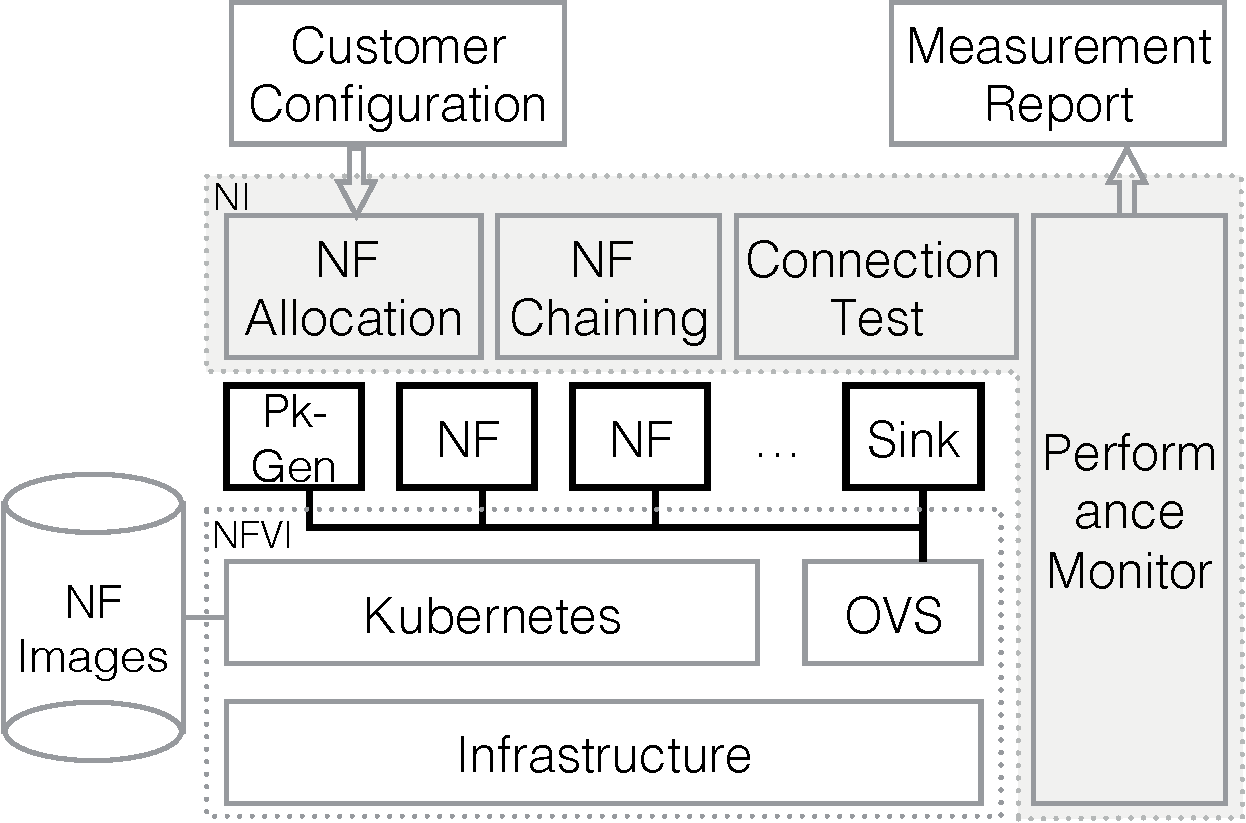
\includegraphics[width=3.3in]{design2.pdf}
\caption{An overview of our benchmark design.}
\label{design}
\end{figure}

%Framework
%for ppl from network field
To achieve the demand of easy to use, 
users are supposed to run only one command to start the test, 
and touch only two files, 
one configuration file and one measurement report. 

The architecture of our benchmark is shown in Figure \ref{design}. 
It has three main parts, NFVI, NF service and NI.
NFVI (NFV Infrastructure) is consisted of hardware resources 
including compute, storage and network. 
NF services are deployed upon NFVI, forming a service chain. 
NI is the key component of our benchmark. 
It does NF allocation and chaining automatically leveraging NFVI management framework.
Furthermore, it does connection test and performance monitoring during test running.
The process to use the benchmark includes five steps: 

\begin{itemize}
\item[\textbf{1.}]{}\textbf{Pre-install} 
In the first step, users need to install Kubernetes, OVS 
and Openflow controller for their physical server cluster. 
Kubernetes is an open-source system for automating deployment, scaling, 
and management of containerized applications. 
To force forwarding packets cross nodes, 
OVS bridge and Openflow global control is needed. 

\item[\textbf{2.}]{}\textbf{Build images} 
We provide DOCKERFILE to build images for each VNF listed in Table \ref{nfs}, 
A private registry is needed to manage the images, 
so that Kubernetes can create containers distributely using local images.

\item[\textbf{3.}]{}\textbf{Write config file} 
This config file is the only file needs user edit. 
It includes choice of testing chain, 
mapping between physical server and docker,
resource configuration of each docker, 
host network and other NF specific configurations. 
To config each NF working in the demanded mode, 
we provide pre-written config files for each NF. 

\item[\textbf{4.}]{}\textbf{One click running} 
Users can run the test by executing only one command. 
NI does a series automate processes. 
First it reads the configuration file edited by users and rewrites the related scripts, 
which including container deployment scripts and NF config files. 
Then the NF Allocation module deploys containers according to user configuration. 
When containers are started and their status turn to `ready', 
NF Chaining module adds virtual NIC for each container, 
connects them to OVS bridge, 
and installs Openflow forwarding rules according to the chaining policy. 
To check whether the chain works, 
the Connection Test module send a TCP request 
from the packet generator and check if it gets response from Apache server. 
If the connection test is passed, 
the test is run and metric measurement begins.

\item[\textbf{5.}]{}\textbf{Get the report} 
The Performance Monitor module does metric measurement 
and output a report.

\end{itemize}

%\section{Implementation}

\section{Evaluation}
We have implemented a demo version of our benchmark. 
It now can work on a single node, 
and measure classic network metrics such as throughput and latency.
In this section, we evaluate two chains in NFVInsight. 
The testbed we used for our evaluation builds on an edge server (Intel Xeon E5V3-2658 2.2GHz, 12 cores, 32GB, 2$\times$1Gbps NICs) that runs CentOS 7 system, with Kubernetes 1.4 and Open vSwitch 2.5.1. We encapsulates NFs with Docker 1.12.5 running Ubuntu 14.14. 

\subsection{Throughput}

%\begin{figure}[t]
%\label{cdf}
%\centering
%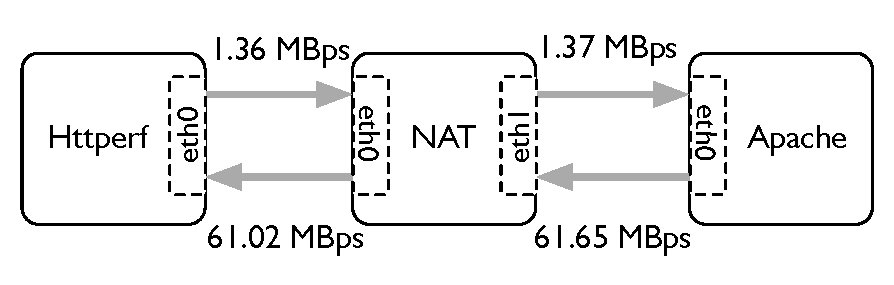
\includegraphics[width=3.3in]{throughput_chain1.eps}
%\caption{Throughput of each NF of SFC1.}
%\end{figure}
%
%\begin{figure}[t]
%\label{cdf}
%\centering
%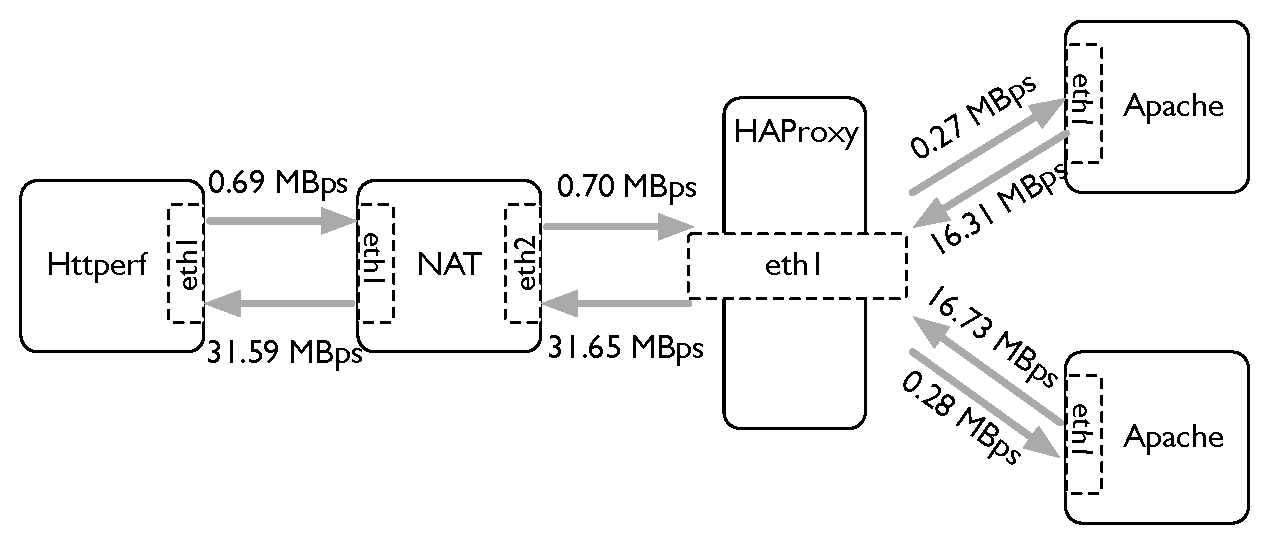
\includegraphics[width=3.3in]{throughput_chain2.eps}
%\caption{Throughput of each NF of SFC2.}
%\end{figure}

\begin{figure}[!t]
\centering
\subfloat[SFC1]{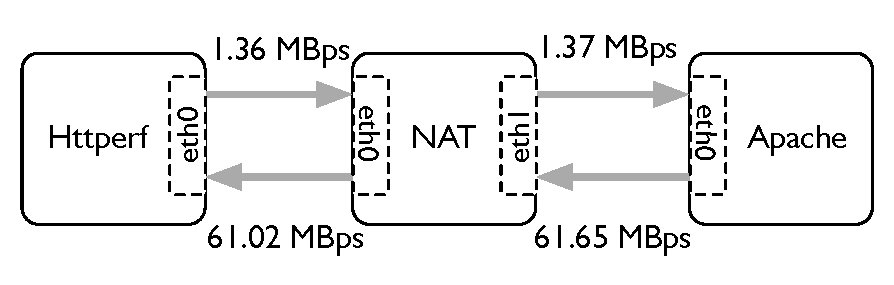
\includegraphics[width=3.3in]{throughput_chain1.eps}
\label{throughput_SFC1}}
\hfil
\subfloat[SFC2]{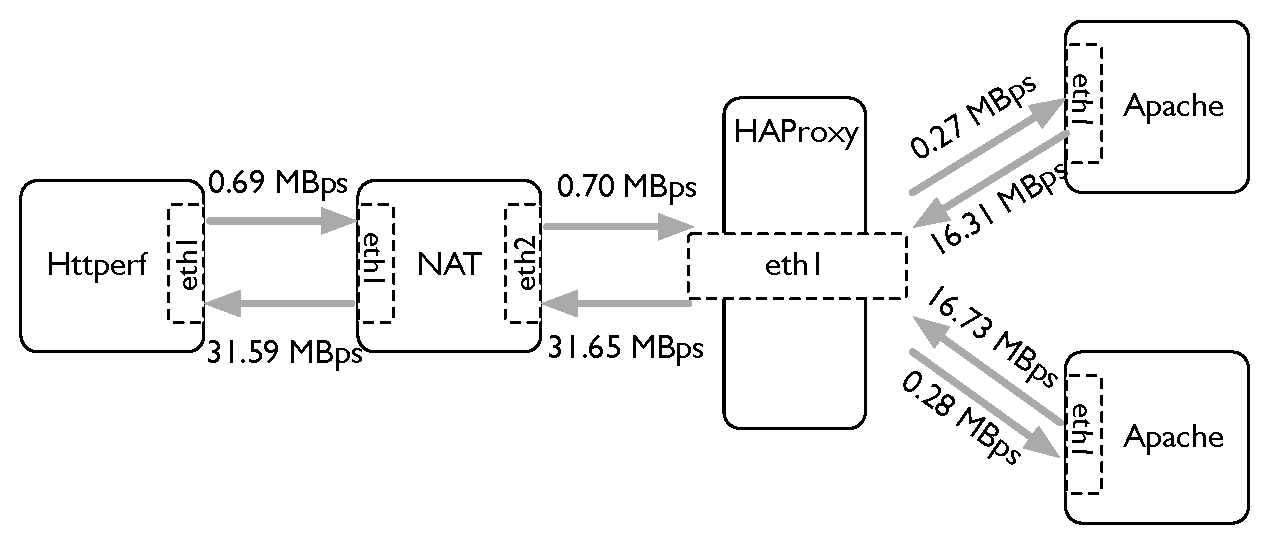
\includegraphics[width=3.3in]{throughput_chain2.eps}
\label{throughput_SFC2}}
\hfil
\caption{Throughput of each NF}
\label{throughput}
\end{figure}

We measure throughput of each container using Docker API. 
The transmit bytes and receive bytes are recorded two times 
at the begin and end of test running respectively. 
Throughput of each NF is calculated 
by doing subtraction of transmit bytes and divid it by the testing time.

Figure \ref{throughput} shows the topology of two chains 
and the throughput labeled on the arrows. 
The throughput is divided by request throughput and respond throughput.

\subsection{Latency}

\begin{figure}[t]
\centering
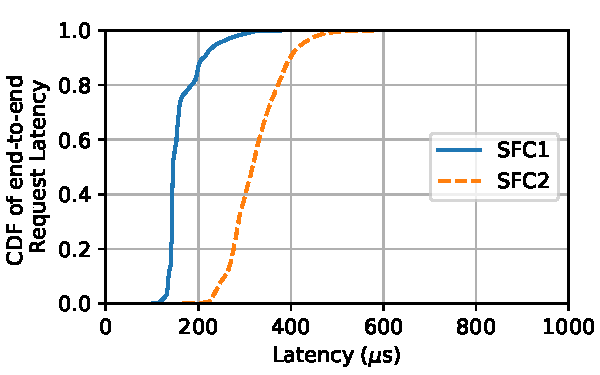
\includegraphics[width=3.3in]{e2e_latency_chain12.pdf}
\caption{End-to-end request latency of SFC1 and SFC2.}
\label{e2e_latency}
\end{figure}

\begin{figure}[t]
\centering
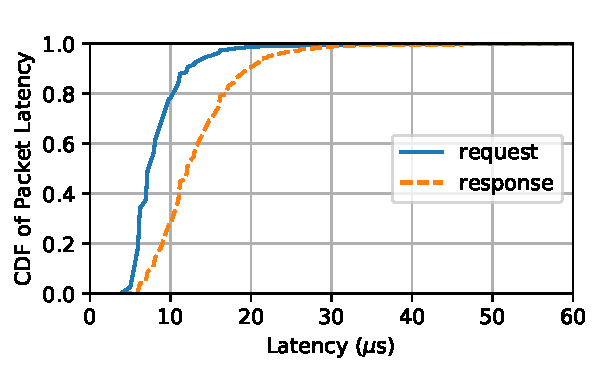
\includegraphics[width=3.3in]{cdf_chain1.pdf}
\caption{Per-packet latency of NAT in SFC1}
\label{nat_latency}
\end{figure}

We modified the workload generator Httperf to output the latency of each request. 
Figure \ref{e2e_latency} shows the end to end latency of SFC1 and SFC2. 
Figure \ref{nat_latency} shows the per-packet latency of NAT in SFC1. 


%\begin{figure}[t]
%\label{cdf}
%\centering
%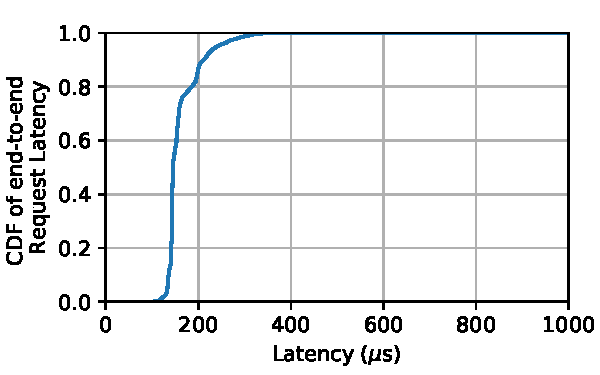
\includegraphics[width=3.3in]{e2e_latency_chain1.pdf}
%\caption{Throughput}
%\end{figure}

%\begin{figure}[t]
%\label{cdf}
%\centering
%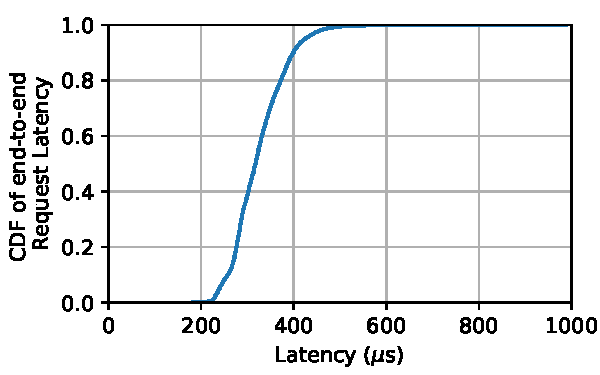
\includegraphics[width=3.3in]{e2e_latency_chain2.pdf}
%\caption{Throughput}
%\end{figure}



%\section{Related Works}
\section{Conclusions}

%\end{document}  % This is where a 'short' article might terminate

%ACKNOWLEDGMENTS are optional
%\section{Acknowledgments}

%
% The following two commands are all you need in the
% initial runs of your .tex file to
% produce the bibliography for the citations in your paper.
\bibliographystyle{abbrv}
\bibliography{NFV_bib,NFV}  
% sigproc.bib is the name of the Bibliography in this case
% You must have a proper ".bib" file
%  and remember to run:
% latex bibtex latex latex
% to resolve all references
%
% ACM needs 'a single self-contained file'!
%
%APPENDICES are optional
%\balancecolumns
%\appendix
%%Appendix A
%\section{Headings in Appendices}
%The rules about hierarchical headings discussed above for
%the body of the article are different in the appendices.
%In the \textbf{appendix} environment, the command
%\textbf{section} is used to
%indicate the start of each Appendix, with alphabetic order
%designation (i.e. the first is A, the second B, etc.) and
%a title (if you include one).  So, if you need
%hierarchical structure
%\textit{within} an Appendix, start with \textbf{subsection} as the
%highest level. Here is an outline of the body of this
%document in Appendix-appropriate form:
%\subsection{Introduction}
%\subsection{The Body of the Paper}
%\subsubsection{Type Changes and  Special Characters}
%\subsubsection{Math Equations}
%\paragraph{Inline (In-text) Equations}
%\paragraph{Display Equations}
%\subsubsection{Citations}
%\subsubsection{Tables}
%\subsubsection{Figures}
%\subsubsection{Theorem-like Constructs}
%\subsubsection*{A Caveat for the \TeX\ Expert}
%\subsection{Conclusions}
%\subsection{Acknowledgments}
%\subsection{Additional Authors}
%This section is inserted by \LaTeX; you do not insert it.
%You just add the names and information in the
%\texttt{{\char'134}additionalauthors} command at the start
%of the document.
%\subsection{References}
%Generated by bibtex from your ~.bib file.  Run latex,
%then bibtex, then latex twice (to resolve references)
%to create the ~.bbl file.  Insert that ~.bbl file into
%the .tex source file and comment out
%the command \texttt{{\char'134}thebibliography}.
%% This next section command marks the start of
%% Appendix B, and does not continue the present hierarchy
%\section{More Help for the Hardy}
%The sig-alternate.cls file itself is chock-full of succinct
%and helpful comments.  If you consider yourself a moderately
%experienced to expert user of \LaTeX, you may find reading
%it useful but please remember not to change it.
%%\balancecolumns % GM June 2007
%% That's all folks!
\end{document}
